% Options for packages loaded elsewhere
% Options for packages loaded elsewhere
\PassOptionsToPackage{unicode}{hyperref}
\PassOptionsToPackage{hyphens}{url}
%
\documentclass[
  ignorenonframetext,
  aspectratio=169,
]{beamer}
\newif\ifbibliography
\usepackage{pgfpages}
\setbeamertemplate{caption}[numbered]
\setbeamertemplate{caption label separator}{: }
\setbeamercolor{caption name}{fg=normal text.fg}
\beamertemplatenavigationsymbolsempty
% remove section numbering
\setbeamertemplate{part page}{
  \centering
  \begin{beamercolorbox}[sep=16pt,center]{part title}
    \usebeamerfont{part title}\insertpart\par
  \end{beamercolorbox}
}
\setbeamertemplate{section page}{
  \centering
  \begin{beamercolorbox}[sep=12pt,center]{section title}
    \usebeamerfont{section title}\insertsection\par
  \end{beamercolorbox}
}
\setbeamertemplate{subsection page}{
  \centering
  \begin{beamercolorbox}[sep=8pt,center]{subsection title}
    \usebeamerfont{subsection title}\insertsubsection\par
  \end{beamercolorbox}
}
% Prevent slide breaks in the middle of a paragraph
\widowpenalties 1 10000
\raggedbottom
\usepackage{iftex}
\ifPDFTeX
  \usepackage[T1]{fontenc}
  \usepackage[utf8]{inputenc}
  \usepackage{textcomp} % provide euro and other symbols
\else % if luatex or xetex
  \usepackage{unicode-math} % this also loads fontspec
  \defaultfontfeatures{Scale=MatchLowercase}
  \defaultfontfeatures[\rmfamily]{Ligatures=TeX,Scale=1}
\fi
\usepackage{lmodern}

\usetheme[]{metropolis}
\ifPDFTeX\else
  % xetex/luatex font selection
\fi
% Use upquote if available, for straight quotes in verbatim environments
\IfFileExists{upquote.sty}{\usepackage{upquote}}{}
\IfFileExists{microtype.sty}{% use microtype if available
  \usepackage[]{microtype}
  \UseMicrotypeSet[protrusion]{basicmath} % disable protrusion for tt fonts
}{}
\makeatletter
\@ifundefined{KOMAClassName}{% if non-KOMA class
  \IfFileExists{parskip.sty}{%
    \usepackage{parskip}
  }{% else
    \setlength{\parindent}{0pt}
    \setlength{\parskip}{6pt plus 2pt minus 1pt}}
}{% if KOMA class
  \KOMAoptions{parskip=half}}
\makeatother


\usepackage{longtable,booktabs,array}
\usepackage{calc} % for calculating minipage widths
\usepackage{caption}
% Make caption package work with longtable
\makeatletter
\def\fnum@table{\tablename~\thetable}
\makeatother
\usepackage{graphicx}
\makeatletter
\newsavebox\pandoc@box
\newcommand*\pandocbounded[1]{% scales image to fit in text height/width
  \sbox\pandoc@box{#1}%
  \Gscale@div\@tempa{\textheight}{\dimexpr\ht\pandoc@box+\dp\pandoc@box\relax}%
  \Gscale@div\@tempb{\linewidth}{\wd\pandoc@box}%
  \ifdim\@tempb\p@<\@tempa\p@\let\@tempa\@tempb\fi% select the smaller of both
  \ifdim\@tempa\p@<\p@\scalebox{\@tempa}{\usebox\pandoc@box}%
  \else\usebox{\pandoc@box}%
  \fi%
}
% Set default figure placement to htbp
\def\fps@figure{htbp}
\makeatother





\setlength{\emergencystretch}{3em} % prevent overfull lines

\providecommand{\tightlist}{%
  \setlength{\itemsep}{0pt}\setlength{\parskip}{0pt}}



 


% ============================================================
%  Econ 2203 — Beamer Metropolis Theme Preamble
%  Course: International Trade and Policy in Agriculture
%  Instructor: Nithin M, Department of Development Economics
% ============================================================

% MUST be first: load Metropolis theme before \metroset and colour overrides
\usetheme{metropolis}

% Only load packages not already provided by pandoc's beamer template
\usepackage{amsmath,amssymb}

% ---- Brand colours -----------------------------------------
\definecolor{brandblue}{HTML}{012169}
\definecolor{brandgold}{HTML}{B9975B}
\definecolor{lightblue}{HTML}{E8EDF5}

% ---- Metropolis colour overrides ---------------------------
% Main palette
\setbeamercolor{normal text}{fg=black,bg=white}
\setbeamercolor{background canvas}{bg=white}
\setbeamercolor{alerted text}{fg=brandgold}
\setbeamercolor{example text}{fg=brandblue!70!black}

% Title slide
\setbeamercolor{title}{fg=white,bg=brandblue}
\setbeamercolor{subtitle}{fg=brandgold}
\setbeamercolor{author}{fg=white}
\setbeamercolor{institute}{fg=brandgold!80!white}
\setbeamercolor{date}{fg=white}
\setbeamercolor{title page header}{fg=white,bg=brandblue}

% Frametitle bar
\setbeamercolor{frametitle}{fg=white,bg=brandblue}

% Progress bar → gold
\setbeamercolor{progress bar}{fg=brandgold,bg=brandblue!30}
\setbeamercolor{title separator}{fg=brandgold}
\setbeamercolor{progress bar in head/foot}{fg=brandgold,bg=brandblue!20}
\setbeamercolor{progress bar in section page}{fg=brandgold,bg=brandblue!20}

% Blocks
\setbeamercolor{block title}{bg=brandblue,fg=white}
\setbeamercolor{block body}{bg=lightblue,fg=black}
\setbeamercolor{block title alerted}{bg=brandgold,fg=white}
\setbeamercolor{block body alerted}{bg=brandgold!12,fg=black}
\setbeamercolor{block title example}{bg=brandblue!70!black,fg=white}
\setbeamercolor{block body example}{bg=brandblue!8,fg=black}

% Structure / lists
\setbeamercolor{structure}{fg=brandblue}
\setbeamercolor{section in toc}{fg=brandblue}
\setbeamercolor{itemize item}{fg=brandblue}
\setbeamercolor{itemize subitem}{fg=brandgold}
\setbeamercolor{enumerate item}{fg=brandblue}
\setbeamercolor{description item}{fg=brandblue}

% ---- Metropolis options ------------------------------------
\metroset{
  progressbar    = frametitle,   % gold bar under frametitle
  sectionpage    = none,
  numbering      = fraction,
  block          = fill
}

% ---- Fonts (Metropolis uses Fira Sans; fallback gracefully) -
\setbeamerfont{title}{size=\Large,series=\bfseries}
\setbeamerfont{subtitle}{size=\normalsize,series=\mdseries}
\setbeamerfont{frametitle}{size=\large,series=\bfseries}
\setbeamerfont{block title}{size=\normalsize,series=\bfseries}
\setbeamerfont{caption}{size=\footnotesize}

% ---- Footer: lecture title + course + slide number ----------
\setbeamertemplate{footline}{%
  \begin{beamercolorbox}[wd=\paperwidth,ht=2.0ex,dp=1ex]{footline}%
    \hspace{0.8em}%
    {\footnotesize\color{brandblue!60}%
      \insertshorttitle
      \hfill Nithin M \hfill
      \insertframenumber{}/\inserttotalframenumber\hspace{0.8em}}%
  \end{beamercolorbox}%
}

% ---- Misc --------------------------------------------------
\setlength{\parskip}{2pt}
\setbeamertemplate{navigation symbols}{}

% tighter column sep for side-by-side content
\setlength{\columnsep}{0.8em}

% ---- Max 6 lines per slide: compact list typesetting -------
% Smaller fonts at each list depth
\setbeamerfont{itemize/enumerate body}{size=\small}
\setbeamerfont{itemize/enumerate subbody}{size=\footnotesize}
\setbeamerfont{itemize/enumerate subsubbody}{size=\scriptsize}

% Tight vertical spacing injected at the start of each list level
\setbeamertemplate{itemize/enumerate body begin}{%
  \setlength{\itemsep}{3pt}\setlength{\parsep}{0pt}}
\setbeamertemplate{itemize/enumerate subbody begin}{%
  \setlength{\itemsep}{2pt}\setlength{\parsep}{0pt}}
\setbeamertemplate{itemize/enumerate subsubbody begin}{%
  \setlength{\itemsep}{1pt}\setlength{\parsep}{0pt}}

% Global safety net: default frame shrink = 10 %
% \beamer@shrinkfalse is called ONCE in beamer's frame init (line 438 of
% beamerbaseframe.sty) before the user's options are processed (line 444).
% By redefining it we inject shrink=10 right after the reset; if the frame
% explicitly specifies [shrink=X], the later \setkeys call overrides it.
\makeatletter
\let\beamer@orig@shrinkfalse\beamer@shrinkfalse
\def\beamer@shrinkfalse{%
  \beamer@orig@shrinkfalse
  \setkeys{beamerframe}{shrink=10}}
\makeatother

% Fix: make \label truly robust in moving arguments.
% Quarto wraps figure labels inside captions; Metropolis expands them
% in batchmode causing a crash. DeclareRobustCommand prevents expansion.
\makeatletter
\let\quarto@originallabel\label
\DeclareRobustCommand*{\label}[1]{\quarto@originallabel{#1}}
\makeatother

% Prevent figures from overflowing Beamer frames.
% width=\linewidth: scale to text width (already Quarto default);
% height=0.6\textheight: cap height so figures never push past the frame bottom.
% keepaspectratio: never distort — whichever constraint binds first wins.
\setkeys{Gin}{width=\linewidth,height=0.55\textheight,keepaspectratio}
\makeatletter
\@ifpackageloaded{caption}{}{\usepackage{caption}}
\AtBeginDocument{%
\ifdefined\contentsname
  \renewcommand*\contentsname{Table of contents}
\else
  \newcommand\contentsname{Table of contents}
\fi
\ifdefined\listfigurename
  \renewcommand*\listfigurename{List of Figures}
\else
  \newcommand\listfigurename{List of Figures}
\fi
\ifdefined\listtablename
  \renewcommand*\listtablename{List of Tables}
\else
  \newcommand\listtablename{List of Tables}
\fi
\ifdefined\figurename
  \renewcommand*\figurename{Figure}
\else
  \newcommand\figurename{Figure}
\fi
\ifdefined\tablename
  \renewcommand*\tablename{Table}
\else
  \newcommand\tablename{Table}
\fi
}
\@ifpackageloaded{float}{}{\usepackage{float}}
\floatstyle{ruled}
\@ifundefined{c@chapter}{\newfloat{codelisting}{h}{lop}}{\newfloat{codelisting}{h}{lop}[chapter]}
\floatname{codelisting}{Listing}
\newcommand*\listoflistings{\listof{codelisting}{List of Listings}}
\makeatother
\makeatletter
\makeatother
\makeatletter
\@ifpackageloaded{caption}{}{\usepackage{caption}}
\@ifpackageloaded{subcaption}{}{\usepackage{subcaption}}
\makeatother

\usepackage{bookmark}
\IfFileExists{xurl.sty}{\usepackage{xurl}}{} % add URL line breaks if available
\urlstyle{same}
\hypersetup{
  pdftitle={Lecture 15: SPS Measures and Codex Alimentarius},
  pdfauthor={Nithin M},
  hidelinks,
  pdfcreator={LaTeX via pandoc}}


\title[L15 \textbar{} SPS \& Codex]{Lecture 15: SPS Measures and Codex
Alimentarius}
\subtitle{Econ 2203 \textbar{} International Trade and Policy in
Agriculture}
\author{Nithin M}
\date{2026-08-01}
\institute{Department of Development Economics}

\begin{document}
\frame{\titlepage}


\begin{frame}{Recap: Lecture 14}
\phantomsection\label{recap-lecture-14}
\textbf{Lecture 14} examined the Agreement on Agriculture -- the WTO
rulebook for farm support and market access.

\begin{columns}[T]
\begin{column}{0.55\linewidth}
\textbf{Key ideas from Lecture 14:}

\begin{itemize}
\tightlist
\item
  Three Pillars: Market Access, Domestic Support, Export Competition
\item
  India's bound tariffs (\textasciitilde113\% average) = policy
  flexibility
\item
  Three Boxes: Green (unlimited), Blue (conditional), Amber (limited)
\item
  India's MSP procurement exceeds de minimis -- protected by Peace
  Clause
\item
  Doha Round dead; permanent solution pending
\end{itemize}
\end{column}

\begin{column}{0.45\linewidth}
\textbf{Today's Bridge}

You now understand that WTO rules govern tariffs and subsidies. But even
if tariffs are zero and subsidies are legal -- goods can still be
blocked at the border.

\textbf{How?} Through food safety and quality standards.

This lecture covers the SPS Agreement and Codex Alimentarius -- the
standards that determine whether Indian agricultural exports can
actually reach foreign consumers.
\end{column}
\end{columns}
\end{frame}

\begin{frame}{Opening Case: The MDH-Everest Spice Scandal}
\phantomsection\label{opening-case-the-mdh-everest-spice-scandal}
\begin{columns}[T]
\begin{column}{0.55\linewidth}
\textbf{April 2023 -- A Crisis for Indian Spice Exports}

\begin{itemize}
\tightlist
\item
  \textbf{Singapore Food Agency} ordered recall of MDH Madras Curry
  Powder and Everest Fish Curry Masala
\item
  \textbf{Hong Kong Centre for Food Safety} recalled MDH and Everest
  products
\item
  \textbf{Maldives} banned imports of specific MDH and Everest products
\item
  EU RASFF (Rapid Alert System for Food and Feed): multiple Indian spice
  alerts triggered
\end{itemize}

\textbf{The violation:} Ethylene oxide (ETO) residue above maximum
permitted levels

\textbf{Ethylene oxide:} A fumigant used to kill bacteria (Salmonella)
and insects in stored spices. Classified as a probable carcinogen.
EU/Singapore MRL: 0.02 mg/kg (effectively zero tolerance).

\textbf{Estimated export disruption:} Tens of millions of dollars;
reputational damage to India's Rs 35,000 crore+ spice export industry
\end{column}

\begin{column}{0.45\linewidth}
\textbf{Why This Happened}

Spices are stored in warehouses and can carry Salmonella. Exporters
fumigated with ETO to ensure microbiological safety -- a common
practice.

But ETO MRLs were tightened in EU and Singapore well below what Indian
producers knew or monitored.

The question: Was this \textbf{genuine food safety} regulation or
\textbf{disguised protectionism}?

Answer: In this case, \textbf{genuine} -- ETO is a real carcinogen; the
standard had scientific basis. But the principle of distinction matters
enormously for WTO disputes.

\textbf{India's Response:} FSSAI banned ETO fumigation for export-bound
spices (2023). Spices Board mandated pre-export testing.
\end{column}
\end{columns}
\end{frame}

\begin{frame}{What Are SPS Measures?}
\phantomsection\label{what-are-sps-measures}
\begin{columns}[T]
\begin{column}{0.55\linewidth}
\textbf{Sanitary and Phytosanitary Measures}

Defined in \textbf{WTO SPS Agreement Annex A}:

\textbf{Sanitary measures:} Protect human or animal life/health from
risks from: - Food additives, contaminants, toxins, pesticide residues -
Veterinary drug residues in food - Diseases carried by animals (FMD,
bird flu, BSE) - Organisms in food (Salmonella, E. coli, Listeria)

\textbf{Phytosanitary measures:} Protect plant health from: - Pests
(locusts, mango seed weevil, citrus greening) - Diseases (wheat rust,
rice blast) - Invasive species through traded plant material
\end{column}

\begin{column}{0.45\linewidth}
\textbf{SPS vs.~TBT: An Important Distinction}

\textbf{SPS Agreement:} Food safety, animal health, plant health

\textbf{TBT Agreement:} All other technical regulations -- labelling,
packaging, environmental standards, sustainability certifications,
organic certification

The distinction matters because: - SPS standards must be
\textbf{scientifically based} (strict discipline) - TBT standards:
``necessary'' to fulfil legitimate objectives, but the scientific
requirement is less strict

When in doubt: food safety measures = SPS; labelling/quality standards =
TBT
\end{column}
\end{columns}
\end{frame}

\begin{frame}
\end{frame}

\section{The WTO SPS Agreement}\label{the-wto-sps-agreement}

\begin{frame}{WTO SPS Agreement: Core Principles}
\phantomsection\label{wto-sps-agreement-core-principles}
\begin{columns}[T]
\begin{column}{0.5\linewidth}
\textbf{Five Key Principles (1995)}

\textbf{1. Right to Protect} Every country has the \textbf{sovereign
right} to set its own level of sanitary and phytosanitary protection --
even above international standards. There is no ``harmonisation''
obligation.

\textbf{2. Scientific Basis (Art. 2)} SPS measures must be based on
scientific principles and not maintained without sufficient scientific
evidence.

\textbf{3. Non-Discrimination (Art. 2)} SPS measures must not
arbitrarily discriminate between countries with similar conditions. If
India is FMD-free in one region, a country should not ban all Indian
meat.
\end{column}

\begin{column}{0.5\linewidth}
\textbf{4. International Standards (Art. 3)} SPS measures based on Codex
Alimentarius / OIE / IPPC standards are \textbf{presumed WTO-consistent}
-- no further justification needed.

If stricter than international standards, the member must conduct a
\textbf{risk assessment} (Art. 5) to justify the higher protection
level.

\textbf{5. Precautionary Principle (Art. 5.7)} When scientific evidence
is insufficient, a member may provisionally adopt SPS measures. Must: -
Seek additional information - Review the measure within a reasonable
time

The SPS Agreement creates a \textbf{two-track system:} align with
Codex/OIE/IPPC (easy compliance) or justify stricter measures with your
own risk assessment (hard but possible).
\end{column}
\end{columns}
\end{frame}

\begin{frame}{Codex Alimentarius and OIE}
\phantomsection\label{codex-alimentarius-and-oie}
\begin{columns}[T]
\begin{column}{0.5\linewidth}
\textbf{Codex Alimentarius Commission (CAC)}

Established: 1963 by FAO and WHO

Covers: \textbf{Food safety} - Maximum Residue Limits (MRLs) for
pesticides - MRLs for veterinary drug residues - Food additive standards
- Contaminant limits (aflatoxins, heavy metals)

188 member countries

\textbf{India:} Founding member; represented by FSSAI
\end{column}

\begin{column}{0.5\linewidth}
\textbf{WOAH (formerly OIE)}

World Organisation for Animal Health

Established: 1924, Paris

Covers: \textbf{Animal health and zoonoses} - Disease status
classification (FMD-free zones, etc.) - International standards for safe
trade of animals - Veterinary medicines - Animal welfare

India is member; uses WOAH standards for import/export conditions on
livestock and livestock products
\end{column}
\end{columns}
\end{frame}

\begin{frame}{IPPC and the SPS Standards Hierarchy}
\phantomsection\label{ippc-and-the-sps-standards-hierarchy}
\begin{columns}[T]
\begin{column}{0.5\linewidth}
\textbf{IPPC}

International Plant Protection Convention

Established: 1952 under FAO

Covers: \textbf{Plant health} - International Standards for
Phytosanitary Measures (ISPMs) - Pest Risk Assessment (PRA) methodology
- Phytosanitary certificates - Treatment protocols (heat, irradiation,
cold)

India's DPPQS (Directorate of Plant Protection) implements IPPC. Issues
phytosanitary certificates for all plant exports.
\end{column}

\begin{column}{0.5\linewidth}
\textbf{SPS Standards Hierarchy}

WTO SPS Agreement Article 3:

\begin{enumerate}
\tightlist
\item
  \textbf{Codex/OIE/IPPC standard} → presumed WTO-consistent; no
  justification needed
\item
  \textbf{More protective than Codex} → permitted \emph{only if} based
  on scientific risk assessment (Art. 5)
\item
  \textbf{Precautionary measures} → temporary; must seek additional
  information for review
\end{enumerate}

\textbf{Two-track system:} - Align with Codex/OIE/IPPC → easy compliance
path - Justify stricter measure with own risk assessment → hard but
possible

India's strategy: ensure products meet Codex standards as baseline, then
challenge stricter import-country standards by demanding risk assessment
justification.
\end{column}
\end{columns}
\end{frame}

\begin{frame}{Codex Alimentarius: How It Works}
\phantomsection\label{codex-alimentarius-how-it-works}
\begin{columns}[T]
\begin{column}{0.55\linewidth}
\textbf{``The Food Code'' -- Setting the Global MRL Standard}

\textbf{Scientific committees behind Codex:}

\begin{itemize}
\item
  \textbf{JMPR} (Joint FAO/WHO Meeting on Pesticide Residues): Evaluates
  pesticides; recommends MRLs. Considers: acceptable daily intake (ADI),
  dietary exposure, good agricultural practice (GAP).
\item
  \textbf{JECFA} (Joint Expert Committee on Food Additives): Evaluates
  food additives and veterinary drug residue limits.
\end{itemize}

\textbf{Process:} Exposure assessment + toxicological evaluation +
dietary intake modeling = proposed MRL

If Codex sets an MRL of \textbf{0.5 mg/kg} for chlorpyrifos in spices,
this becomes the international benchmark.
\end{column}

\begin{column}{0.45\linewidth}
\textbf{Why Codex Standards Matter for India}

If India's exports comply with \textbf{Codex MRLs}, no WTO member can
block them on SPS grounds \textbf{without doing their own risk
assessment}.

If an importing country sets a stricter standard than Codex (e.g., EU's
0.01 mg/kg for many pesticides), they must provide: 1. A scientific risk
assessment 2. Evidence that the Codex standard does not achieve their
chosen protection level

Many EU standards pass this test (precautionary approach). Some may not
-- creating WTO dispute opportunities.

India's strategy: ensure Indian products meet \textbf{Codex standards}
as the baseline. Then challenge importing country standards stricter
than Codex by demanding the risk assessment justification.
\end{column}
\end{columns}
\end{frame}

\begin{frame}{Codex Alimentarius: Standards Portfolio}
\phantomsection\label{codex-alimentarius-standards-portfolio}
\begin{figure}

\centering{

\pandocbounded{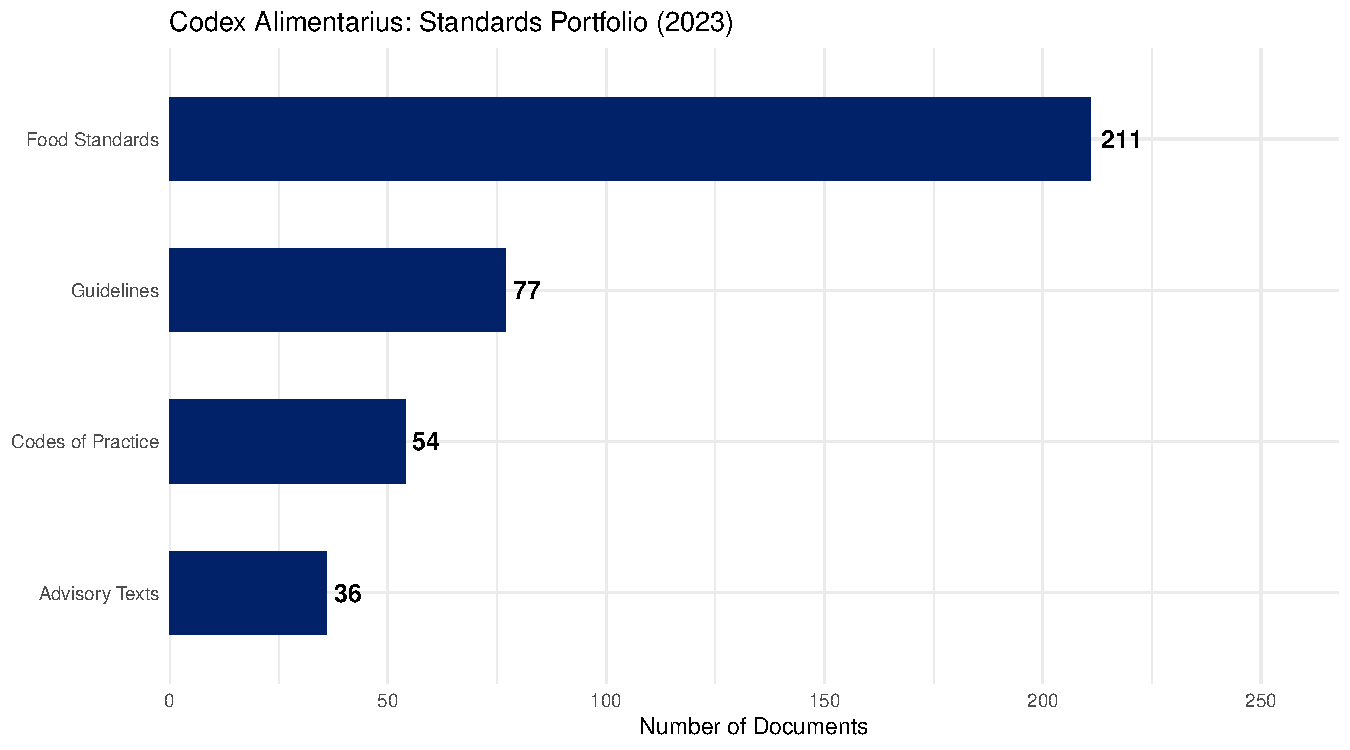
\includegraphics[keepaspectratio]{Lecture15_SPS_Codex_files/figure-beamer/fig-codex-standards-1.pdf}}

}

\caption{Codex Alimentarius: Standards
Portfolio (2023) Source: Codex Alimentarius Commission, FAO/WHO.}
\label{fig-codex-standards}

\end{figure}%
\end{frame}

\begin{frame}{FSSAI: India's Food Safety Regulator}
\phantomsection\label{fssai-indias-food-safety-regulator}
\begin{columns}[T]
\begin{column}{0.55\linewidth}
\textbf{Food Safety and Standards Authority of India}

Established under the FSSAI Act, 2006 (fully operational 2011).
Headquarters: New Delhi.

\textbf{FSSAI's Roles:}

\begin{itemize}
\tightlist
\item
  Sets food safety standards for domestic market
\item
  India's national Codex Contact Point
\item
  Accredits food testing laboratories (NABL)
\item
  Issues export health certificates (through EIC for many products)
\item
  Regulates food businesses (importers, processors, retailers)
\item
  Runs FoSTaC (Food Safety Training and Certification)
\end{itemize}

\textbf{Recent FSSAI actions on SPS compliance:} - Updated pesticide
MRLs for 200+ pesticides (2023) - Banned ETO fumigation for export-bound
spices - Harmonised aflatoxin limits with Codex (15 ppb for food, 10 ppb
for baby food) - Launched FSSAI Food Safety Connect portal for exporters
\end{column}

\begin{column}{0.45\linewidth}
\textbf{Gap Between FSSAI and Import Country Standards}

Some FSSAI standards are \textbf{still below Codex} or \textbf{more
permissive than importing country standards}:

\begin{itemize}
\tightlist
\item
  Pesticide MRLs: FSSAI covers \textasciitilde320 pesticides; Indian
  farmers use 300+ pesticides. Gaps exist.
\item
  Aflatoxin limits in spices: FSSAI = 15 ppb; EU = 10 ppb; Japan = 10
  ppb
\item
  Veterinary drug residues: FSSAI has fewer VMDRs than Codex
\end{itemize}

\textbf{The compliance challenge:} Indian exporters must meet the
\textbf{importing country's standard} (or Codex if importing country has
none) -- not just FSSAI's domestic standard
\end{column}
\end{columns}
\end{frame}

\begin{frame}{India's SPS export challenges (examples I)}
\phantomsection\label{indias-sps-export-challenges-examples-i}
\begin{itemize}
\tightlist
\item
  \textbf{Spices:} ETO / pesticide residues / aflatoxin (EU, Singapore,
  USA)
\item
  \textbf{Marine products:} antibiotic residues, Salmonella (USA, EU,
  Japan)
\item
  \textbf{Rice:} pesticide MRLs (EU)
\item
  \textbf{Fresh grapes:} pesticide MRLs (EU)
\item
  \textbf{Mangoes:} pest risks (USA, Japan, Korea)
\end{itemize}
\end{frame}

\begin{frame}{India's SPS export challenges (examples II)}
\phantomsection\label{indias-sps-export-challenges-examples-ii}
\begin{itemize}
\tightlist
\item
  \textbf{Peanuts:} aflatoxin (EU)
\item
  \textbf{Buffalo meat:} veterinary residues; animal health (Gulf, SEA)
\item
  \textbf{Honey:} antibiotics and pesticide contamination (EU, USA)
\item
  Common pattern: \textbf{lab testing + traceability + farm practices}
  must align
\item
  SPS barriers often bite hardest in \textbf{premium markets}
\end{itemize}
\end{frame}

\begin{frame}{Scale: why SPS matters for India}
\phantomsection\label{scale-why-sps-matters-for-india}
\begin{itemize}
\tightlist
\item
  Agri exports (2023--24): about \textbf{\$50B}
\item
  High-exposure earners: \textbf{rice, marine, spices, buffalo meat}
\item
  EU RASFF alerts on India-origin products: \textbf{200+ per year}
\item
  US FDA import refusals: India often ranks \textbf{3rd--5th}
\item
  Takeaway: SPS is a major \textbf{non-tariff barrier} for export growth
\end{itemize}
\end{frame}

\begin{frame}{EU RASFF Alerts on Indian Food Products}
\phantomsection\label{eu-rasff-alerts-on-indian-food-products}
\begin{figure}

\centering{

\pandocbounded{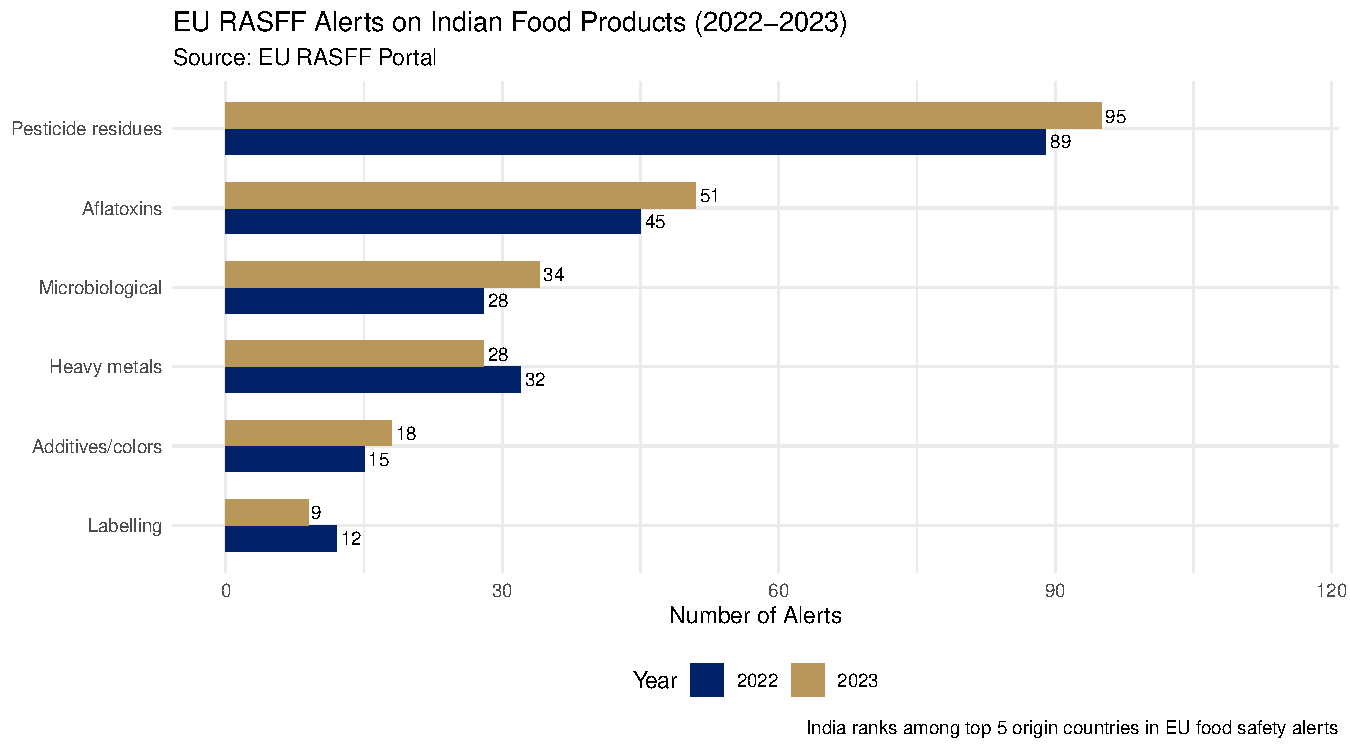
\includegraphics[keepaspectratio]{Lecture15_SPS_Codex_files/figure-beamer/fig-eu-rasff-1.pdf}}

}

\caption{EU RASFF Alerts on Indian Food Products
(2022-2023) Source: European Commission, RASFF Portal (2023).}
\label{fig-eu-rasff}

\end{figure}%
\end{frame}

\begin{frame}{Case Study 1: Spice Rejections 2023-24}
\phantomsection\label{case-study-1-spice-rejections-2023-24}
\begin{columns}[T]
\begin{column}{0.55\linewidth}
\textbf{The Ethylene Oxide (ETO) Problem}

\textbf{What is ETO?} An industrial chemical used to fumigate spices --
kills bacteria (especially Salmonella), moulds, and insects in bulk
stored spices.

\textbf{Why used:} Spices are dried agricultural products; moisture
during storage leads to Salmonella and aflatoxin. ETO is effective.

\textbf{The problem:} ETO is a Group 1 carcinogen (IARC). When used on
food, residues remain. EU and Singapore: MRL = \textbf{0.02 mg/kg}
(effectively zero).

\textbf{Detection:} EU systematically tests Indian spices since 2020.
Found ETO residues 5-20x above MRL in multiple consignments.
\end{column}

\begin{column}{0.45\linewidth}
\textbf{Supply Chain Analysis}

Where does ETO enter? - Usually at fumigation stage: large warehouses,
cold storage facilities, export consolidation points - NOT at the farm
level

Why did exporters use it? - Salmonella contamination is a real risk --
and causes EU rejections too - ETO was commonly used internationally
until MRLs were tightened - Indian exporters were slow to adapt to EU's
tightening

\textbf{India's corrective actions:} - FSSAI: ETO use prohibited for
export spices - Spices Board: GAP training to 500,000 farmers -
Mandatory pre-export testing at NABL-accredited labs - Cold
disinfestation and steam treatment as alternatives
\end{column}
\end{columns}
\end{frame}

\begin{frame}{Reasons for Spice Export Rejections}
\phantomsection\label{reasons-for-spice-export-rejections}
\begin{figure}

\centering{

\pandocbounded{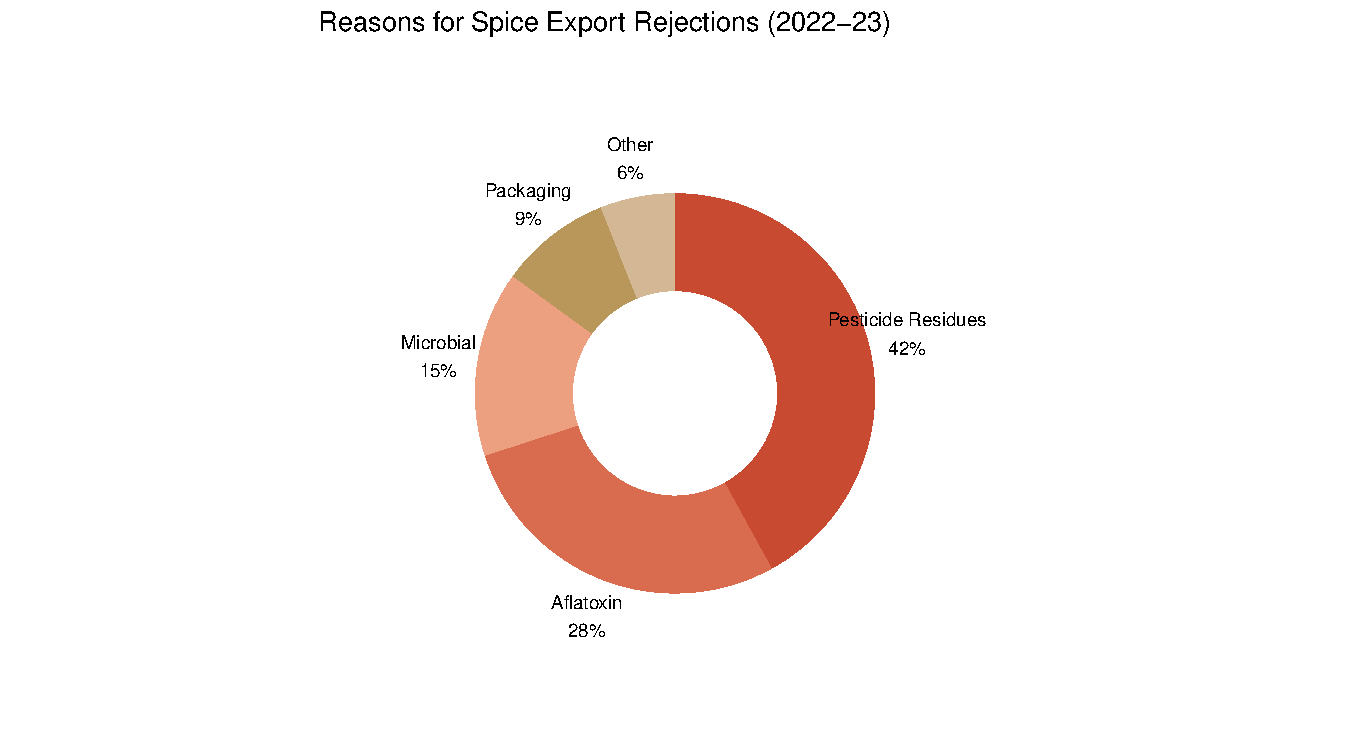
\includegraphics[keepaspectratio]{Lecture15_SPS_Codex_files/figure-beamer/fig-spice-rejection-donut-1.pdf}}

}

\caption{Reasons for Spice Export
Rejections (2022-23) Source: Spices Board India; FSSAI.}
\label{fig-spice-rejection-donut}

\end{figure}%
\end{frame}

\begin{frame}{Case Study 2: Indian Shrimp in the USA}
\phantomsection\label{case-study-2-indian-shrimp-in-the-usa}
\begin{columns}[T]
\begin{column}{0.55\linewidth}
\textbf{India: World's Largest Shrimp Exporter (since 2012)}

India exported \textbf{USD 4.0 billion} of seafood to the USA in 2023
(world's top destination).

\textbf{The Antibiotic Residue Problem}

Shrimp aquaculture uses antibiotics to: - Prevent bacterial diseases
(Vibrio, Aeromonas) - Improve survival rates in intensive ponds

USA/EU banned antibiotics in food animals: - \textbf{Chloramphenicol:}
Carcinogen; zero tolerance (0.3 ppb) -- FDA automatic detention -
\textbf{Nitrofurans (furazolidone):} Zero tolerance -
\textbf{Oxytetracycline:} 2 ppm limit

Indian shrimp occasionally tested positive -- triggering FDA import
alerts and automatic detention of entire shipments from affected
companies.
\end{column}

\begin{column}{0.45\linewidth}
\textbf{India's Response: The MPEDA System}

Marine Products Export Development Authority (MPEDA) created the
\textbf{National Residue Control Plan (NRCP):}

\begin{itemize}
\tightlist
\item
  Farm-level testing before harvest
\item
  MPEDA labs in all major shrimp states (AP, Telangana, Odisha, Gujarat,
  WB)
\item
  Third-party certification (BAP, ASC, GlobalGAP)
\item
  Antibiotic-free certification programs
\item
  Traceability: farm to fork (pond to export container)
\end{itemize}

\textbf{Result:} FDA removed India from ``automatic detention'' list for
most companies (2015). Trust gradually rebuilt.

India's shrimp industry serves as a model of SPS compliance improvement:
investment in testing, traceability, and farmer training
\textbf{converted a crisis into market dominance}. 50\% of US shrimp
imports are from India.
\end{column}
\end{columns}
\end{frame}

\begin{frame}{Case Study 3: Basmati Rice and EU Pesticide Limits}
\phantomsection\label{case-study-3-basmati-rice-and-eu-pesticide-limits}
\begin{columns}[T]
\begin{column}{0.55\linewidth}
\textbf{India's Rice Export Profile}

\begin{itemize}
\tightlist
\item
  India: world's largest rice exporter (\textasciitilde40\% of global
  trade, 2022)
\item
  Basmati: premium segment; EU, Middle East, UK
\item
  Non-basmati: Africa, Bangladesh, Philippines
\end{itemize}

\textbf{The Tricyclazole Problem}

Tricyclazole: fungicide used against rice blast disease (Pyricularia
oryzae). Very effective; widely used in Indian paddy cultivation.

EU MRL for tricyclazole in rice (2016): \textbf{0.01 mg/kg} (This is the
EU ``default'' MRL = lowest measurable limit = effectively zero)

Codex MRL for tricyclazole in rice: \textbf{1 mg/kg} (100x higher)

EU's justification: EFSA (EU food safety body) could not establish an
Acceptable Daily Intake (ADI) for tricyclazole -- so zero tolerance
applied.
\end{column}

\begin{column}{0.45\linewidth}
\textbf{Impact on India}

EU non-basmati rice imports from India: severely restricted since 2016

Basmati: APEDA monitoring programme required farmers to avoid
tricyclazole before harvest. Shift to alternative fungicides
(propiconazole, azoxystrobin).

\textbf{The WTO question:} Is EU's 0.01 mg/kg standard WTO-consistent?

Arguments: - EU: EFSA risk assessment shows no safe ADI = justified
precaution (Art. 5.7) - India: Codex JMPR reviewed same data and set 1
mg/kg; EU is being protectionist

India has raised this at \textbf{WTO SPS Committee} (formal concern
registered)

\textbf{Lesson:} Indian farmers must change agronomic practices to meet
importing country standards. This requires extension services,
alternative pest management, and R\&D for substitute fungicides.
\end{column}
\end{columns}
\end{frame}

\begin{frame}{Animal Health: WOAH Standards and India}
\phantomsection\label{animal-health-woah-standards-and-india}
\begin{columns}[T]
\begin{column}{0.55\linewidth}
\textbf{Foot and Mouth Disease (FMD): India's Biggest Constraint}

India is \textbf{FMD endemic} -- the virus circulates in cattle and
buffalo populations.

Impact: India cannot export fresh/chilled beef and pork to: - EU
(requires FMD-free zone certification) - USA (FMD-free requirement) -
Australia, New Zealand - Japan, South Korea

India CAN export to: - Gulf countries (accept FMD+ origin with
inspection) - Southeast Asia (some countries) - Africa (mainly frozen
buffalo meat)

India is the world's \textbf{largest buffalo meat exporter} (USD 3.5B)
but limited to markets that accept FMD-present-country products. Premium
markets (EU, USA, Japan) are closed.
\end{column}

\begin{column}{0.45\linewidth}
\textbf{India's FMD Control Programme}

\textbf{National Animal Disease Control Programme (NADCP):} - Launched
2019 - Rs 13,300 crore budget - Target: 100\% vaccination of cattle and
buffalo - Goal: FMD-free status by 2025 (revised to 2030) - Brucellosis
control component

\textbf{If India achieves FMD-free zone status:} Could export chilled
beef/pork to EU, Japan -- massive export opportunity (India has world's
largest cattle population: 193 million)

\textbf{WTO Dispute DS430 (India-Agricultural Products):} USA challenged
India's ban on US poultry due to Highly Pathogenic Avian Influenza
(HPAI). India lost -- its HPAI measures were found to violate SPS Art. 5
(not based on proper risk assessment). India had to modify import
protocols.
\end{column}
\end{columns}
\end{frame}

\begin{frame}{IPPC and Plant Quarantine: Mangoes to the USA}
\phantomsection\label{ippc-and-plant-quarantine-mangoes-to-the-usa}
\begin{columns}[T]
\begin{column}{0.55\linewidth}
\textbf{The Mango Market Access Challenge}

India is world's largest mango producer (\textasciitilde55\% of global
output). Yet India barely exports mangoes to the USA and Japan.

\textbf{Why?} Phytosanitary barriers.

\textbf{Mango Seed Weevil} (Sternochetus mangiferae): Lives inside mango
seed; not detectable by visual inspection. USA APHIS requires zero
tolerance -- if present in any consignment, entire shipment rejected and
market access reviewed.

\textbf{USA's phytosanitary protocol:} Vapor Heat Treatment (VHT) -
Mango heated to internal fruit temperature of \textbf{47.2 degrees C for
20 minutes} - Kills all pests including seed weevil - Expensive:
requires VHT chambers at packing houses
\end{column}

\begin{column}{0.45\linewidth}
\textbf{Bilateral Protocol Negotiation}

VHT for mango exports to USA was negotiated bilaterally between: -
India's DPPQS (plant quarantine) - USA's APHIS (Animal and Plant Health
Inspection Service)

India invested in VHT facilities in Maharashtra, Uttar Pradesh, Andhra
Pradesh.

\textbf{Result:} Indian Alphonso, Kesar, and other varieties now
exported to USA (\textasciitilde5,000-8,000 MT/year). Still tiny
vs.~production potential.

\textbf{Japan protocol:} Irradiation treatment (200 Gy gamma/X-ray)
accepted. Facilities limited.

Phytosanitary protocols are \textbf{negotiated product-by-product,
country-by-country}. India must negotiate 50+ protocols for 20+
products. Slow, expensive, but essential for premium market access.
\end{column}
\end{columns}
\end{frame}

\begin{frame}{TBT Agreement: Beyond Food Safety}
\phantomsection\label{tbt-agreement-beyond-food-safety}
\begin{columns}[T]
\begin{column}{0.5\linewidth}
\textbf{Technical Barriers to Trade (TBT Agreement)}

TBT covers standards and regulations NOT related to food
safety/animal-plant health: - Labelling requirements - Packaging
regulations - Environmental standards - Sustainability certifications -
Organic certification - Carbon footprint disclosure

\textbf{Examples affecting India's agri exports:}

\begin{itemize}
\tightlist
\item
  EU ban on single-use plastics: affects packaging of Indian processed
  foods
\item
  EU organic regulation (EU 834/2007): India must have bilateral
  equivalency agreement -- FSSAI-EU organic equivalency being
  renegotiated
\item
  Halal certification: Gulf markets require halal for meat, poultry, and
  some processed foods
\end{itemize}
\end{column}

\begin{column}{0.5\linewidth}
\textbf{EU Carbon Border Adjustment Mechanism (CBAM) -- Emerging TBT/SPS
Challenge}

CBAM (fully operational 2026) requires carbon certificates for imports
of cement, steel, aluminium, fertilisers, electricity, hydrogen.

\textbf{Not directly on food} -- yet. But EU ``Farm to Fork'' strategy
and sustainability standards could extend to agricultural products.

Potential future barriers: - Mandatory deforestation-free certification
(EU Deforestation Regulation -- EUDR) - Supply chain transparency
requirements (traceability, QR codes, blockchain) - Carbon footprint
labelling for food products

India must engage proactively with these emerging standards before they
become barriers.
\end{column}
\end{columns}
\end{frame}

\begin{frame}{Equivalence and Mutual Recognition}
\phantomsection\label{equivalence-and-mutual-recognition}
\begin{columns}[T]
\begin{column}{0.55\linewidth}
\textbf{WTO SPS Article 4: Equivalence}

``Members shall accept the sanitary or phytosanitary measures of other
Members as equivalent, even if these measures differ from their own or
from those used by other Members trading in the same product, if the
exporting Member objectively demonstrates to the importing Member that
its measures achieve the importing Member's appropriate level of
sanitary or phytosanitary protection.''

\textbf{In plain language:} If India can prove that FSSAI's food safety
system achieves the same level of consumer protection as EU's EFSA, EU
should accept Indian food without retesting.

This is very difficult in practice -- few equivalence agreements exist
globally.
\end{column}

\begin{column}{0.45\linewidth}
\textbf{India's Equivalence Arrangements}

\textbf{Achieved:} - \textbf{India-USA Organic Equivalency:} FSSAI
organic standards recognised as equivalent to USDA NOP for specific
products (2012) - \textbf{Japan-India VHT:} Vapor heat protocol =
phytosanitary equivalence for mango - \textbf{EU-India:} Health
certificate arrangements for marine products (not full equivalence)

\textbf{Ongoing negotiations:} - India-EU organic equivalency renewal -
India-UK post-Brexit food safety arrangements (FSSAI-FSA)

Mutual Recognition Agreements (MRAs) reduce compliance costs
dramatically for Indian exporters -- but require India's standards to be
\textbf{demonstrably equivalent} to importing country standards. This is
the strongest incentive for FSSAI modernisation.
\end{column}
\end{columns}
\end{frame}

\begin{frame}{SPS Compliance Costs for India}
\phantomsection\label{sps-compliance-costs-for-india}
\begin{columns}[T]
\begin{column}{0.55\linewidth}
\textbf{Who Bears the Cost of Compliance?}

SPS compliance is \textbf{expensive} -- particularly for developing
countries:

\textbf{Typical compliance costs:}

\begin{itemize}
\tightlist
\item
  \textbf{Laboratory testing:} Rs 1,500-5,000 per consignment (pesticide
  residue panel = 40+ compounds)
\item
  \textbf{Cold chain:} Rs 5-8 per kg for temperature-sensitive products
\item
  \textbf{Certification:} EIC health certificate = Rs 2,500-10,000 per
  consignment
\item
  \textbf{Pre-export testing:} Spices Board mandated ETO test = Rs
  2,000/sample
\item
  \textbf{Third-party certification} (BAP, ASC, GlobalGAP): Rs
  50,000-2,00,000 per farm/facility per year
\item
  \textbf{VHT facility} construction: Rs 5-10 crore per facility
\end{itemize}

\textbf{India's annual SPS compliance infrastructure cost (agri
exports): estimated Rs 500-800 crore}
\end{column}

\begin{column}{0.45\linewidth}
\textbf{India's Testing Infrastructure}

\textbf{NABL-accredited food testing labs:} 200+ (growing rapidly)

Key labs: - \textbf{EIC (Export Inspection Council):} Regional labs in
Chennai, Mumbai, Kolkata, Kochi, Delhi - \textbf{APEDA:} Residue
monitoring programme; 6 regional labs - \textbf{MPEDA:} Aquaculture
testing labs in Nellore, Bhubaneswar, Chennai - \textbf{Spices Board:}
Testing laboratory in Cochin

\textbf{WTO technical assistance:} SPS Agreement provides for capacity
building; FAO/WHO Codex Trust Fund supports developing country
participation in Codex meetings.

Small exporters and farmers bear proportionally higher compliance costs
-- this creates a structural disadvantage for India's fragmented
agricultural sector
\end{column}
\end{columns}
\end{frame}

\begin{frame}{India's Comprehensive SPS Strategy}
\phantomsection\label{indias-comprehensive-sps-strategy}
\textbf{A Six-Pillar Strategy:}

\begin{itemize}
\tightlist
\item
  \textbf{(a) Prevention:} GAP training (Spices Board, APEDA), IPM,
  farmer training on pre-harvest intervals, food safety culture (FSSAI
  Eat Right India)
\item
  \textbf{(b) Detection:} NABL lab accreditation, real-time RASFF
  monitoring, FSSAI surveillance, pre-shipment testing mandates (EIC,
  Spices Board, MPEDA)
\item
  \textbf{(c) Certification:} FSSAI-accredited labs, EIC health
  certificates, third-party international certifications
\item
  \textbf{(d) Bilateral Negotiation:} Phytosanitary protocols
  (product-by-product), equivalence agreements, bilateral veterinary
  certificates
\item
  \textbf{(e) WTO Advocacy:} Register Specific Trade Concerns (STCs) at
  WTO SPS Committee; challenge scientifically unjustified standards
\end{itemize}

\note{\textbf{(f) Domestic Policy:} - FSSAI alignment with Codex -
Pesticide deregistration (remove banned pesticides from Indian market)}
\end{frame}

\begin{frame}{The NTB Dilemma: Safety vs Protectionism}
\phantomsection\label{the-ntb-dilemma-safety-vs-protectionism}
\begin{columns}[T]
\begin{column}{0.55\linewidth}
\textbf{Genuine Food Safety Standard or Disguised Protectionism?}

WTO SPS Agreement: Standards must be: - \textbf{Scientifically based}
(risk assessment, not arbitrary) - \textbf{Non-discriminatory} (same
standard for all origins) - \textbf{Not more trade-restrictive than
necessary} to achieve the protection level

\textbf{Likely genuine:} - EU tricyclazole 0.01 mg/kg (EFSA could not
establish ADI -- precautionary basis has scientific merit even if
contested) - USA zero tolerance for chloramphenicol (carcinogen: no safe
level argument) - Japan's fumigation-free requirements for some products
(genuine pest risk from tropical insects)
\end{column}

\begin{column}{0.45\linewidth}
\textbf{Possible disguised NTBs:} - EU's very strict aflatoxin limit (10
ppb vs.~Codex 15 ppb) in spices: contested whether the marginal health
benefit justifies trade restriction - Japan's requirement for
irradiation treatment for mangoes (alternatives available, less
trade-restricting) - Some EUDR (Deforestation Regulation) product scope
interpretations that could target Indian cotton and soy

\textbf{India's WTO tool:} Register Specific Trade Concerns (STCs) at
the WTO SPS Committee. 59 STCs registered against EU measures -- India
has raised several.

The \textbf{burden of proof} under SPS Agreement: If a measure is
consistent with Codex, importer need not justify. If stricter than
Codex, \textbf{importer must provide risk assessment}. This is India's
legal weapon.
\end{column}
\end{columns}
\end{frame}

\begin{frame}{Emerging SPS/TBT Challenges for India}
\phantomsection\label{emerging-spstbt-challenges-for-india}
\begin{columns}[T]
\begin{column}{0.55\linewidth}
\textbf{The Next Wave of Standards}

\textbf{Antimicrobial Resistance (AMR)} WHO declared AMR a global health
threat. Future measures: - Strict limits on antibiotic use in livestock
and aquaculture - Mandatory AMR monitoring as export condition - India's
National Action Plan on AMR (2017-2021) needs renewal and stronger
implementation

\textbf{EU Deforestation Regulation (EUDR, 2025)} No
deforestation-linked products after Dec 2020. Affects: - Soy (used in
Indian poultry feed chains) - Cattle products from some regions -
Possibly cocoa, coffee from India

Requires geo-referenced supply chain data. Huge compliance investment.
\end{column}

\begin{column}{0.45\linewidth}
\textbf{Digital Traceability}

EU Farm to Fork strategy requires: - QR codes linking product to farm of
origin - Blockchain-based supply chain records - Real-time pesticide
usage data

India's infrastructure: APEDA E-cert, Spices Board TraQiS, MPEDA
Tracenet. Coverage: \textasciitilde30-40\% of exports.

\textbf{Carbon Footprint Labelling}

EU exploring mandatory carbon labels on food products. This would
require Life Cycle Assessment (LCA) data for Indian agricultural
products -- enormous capacity gap.

India must invest NOW in digital traceability, AMR surveillance, and
carbon accounting infrastructure -- or face the next generation of
SPS/TBT barriers when they become mandatory (2025-2030 horizon)
\end{column}
\end{columns}
\end{frame}

\begin{frame}{Key Takeaways: SPS Measures and Codex}
\phantomsection\label{key-takeaways-sps-measures-and-codex}
\textbf{Six Things to Remember from Lecture 15}

\begin{enumerate}
\item
  \textbf{SPS measures are the most important NTB} for India's
  agricultural exports -- more critical than tariffs in premium markets
  (EU, USA, Japan). Annual agri exports at risk: USD 20+ billion.
\item
  \textbf{Codex/OIE/IPPC set the international standard} -- measures
  aligned with these are presumed WTO-consistent. India should ensure
  its products meet Codex MRLs as the minimum standard.
\item
  \textbf{Scientific basis is mandatory} -- if an importing country's
  standard is stricter than Codex, it must conduct a risk assessment.
  This is India's WTO legal tool against possible disguised NTBs.
\item
  \textbf{Investment in compliance infrastructure pays off:} India's
  shrimp industry rebuilt trust with the USA through NRCP and
  third-party certification. Spices industry learning the same lesson
  post-ETO crisis.
\item
  \textbf{Phytosanitary protocols must be negotiated bilaterally} --
  product-by-product, country-by-country. India needs dedicated
  resources for this slow but essential process.
\item
  \textbf{Emerging challenges (AMR, digital traceability, EUDR, carbon
  footprint)} require proactive investment now -- not reactive crisis
  management after export bans.
\end{enumerate}
\end{frame}

\begin{frame}{Next Lecture: Export Procedures and Documentation}
\phantomsection\label{next-lecture-export-procedures-and-documentation}
\begin{columns}[T]
\begin{column}{0.6\linewidth}
\textbf{Lecture 16 (August 11, 2026):}

\textbf{Export Procedures and Documentation}

Turning India's agricultural comparative advantage into actual export
earnings-- the practical mechanics.

We will cover:

\begin{itemize}
\tightlist
\item
  \textbf{Export documentation:} IEC, shipping bill, certificate of
  origin, phytosanitary certificate, health certificate
\item
  \textbf{Export financing:} pre-shipment and post-shipment credit, ECGC
  insurance
\item
  \textbf{Export promotion bodies:} APEDA, MPEDA, Spices Board, Tea
  Board
\item
  \textbf{Port procedures:} customs clearance, inspection,
  containerisation
\item
  \textbf{Case study:} Exporting Alphonso mangoes to the EU from Nashik
  to Rotterdam
\end{itemize}
\end{column}

\begin{column}{0.4\linewidth}
\textbf{A Thought Experiment}

You are a farmer in Nashik with 10 tonnes of Alphonso mangoes ready for
export to the Netherlands.

\emph{What documents do you need? What inspections? What organisations
do you deal with? How is the payment made? What can go wrong?}

Lecture 16 walks through every step of this journey -- from the orchard
gate to the Rotterdam supermarket shelf.

\textbf{Reading:} - APEDA: Export Procedures for Fresh Fruits and
Vegetables - DGFT: Foreign Trade Policy 2023-28 (Chapter 3: Export
Promotion) - RBI: Master Direction on Export of Goods and Services
\end{column}
\end{columns}
\end{frame}

\section{Appendix}\label{appendix}

\begin{frame}{Additional Resources}
\phantomsection\label{additional-resources}
\begin{columns}[T]
\begin{column}{0.5\linewidth}
\textbf{Further Reading}

\begin{itemize}
\tightlist
\item
  Lecture notes and APEDA/WTO official documents
\item
  FSSAI: Food Safety Standards Authority of India
\item
  RBI/DGCI\&S/APEDA databases for latest data
\end{itemize}
\end{column}

\begin{column}{0.5\linewidth}
\textbf{Key Data Sources}

\begin{itemize}
\tightlist
\item
  DGCI\&S: India's merchandise trade
\item
  RBI: Balance of payments data\\
\item
  APEDA: Agricultural export statistics
\item
  WTO: Tariff and trade databases
\end{itemize}
\end{column}
\end{columns}
\end{frame}




\end{document}
